\section{The Lead That Wouldn't Die}
\begin{marginfigure}
\begin{tikzpicture}
\node [name-dest] (box){%
    \begin{minipage}{0.80\textwidth}
    \begin{itemize}
    \item Rhys Tyers
    \item Ben Honan
    \end{itemize}
    \end{minipage}
};
\node[fancytitle, right=10pt] at (box.north west) {Fenestrator};
\end{tikzpicture}
\end{marginfigure}

All year a particular lead had played at my mind. \passage[cave]{Primadona} is still a bit unknown to us, we had only visited one very small branch last year, and so we have little to go on but the drawn survey. Mostly drawn by people who had never been there and based on creatively acquired surveyed data. However someone had drawn an undescended shaft. It looked like it could be 10m wide, and had no bottom drawn on so presumable a few hundred metres of pitch was sure to follow. The navigation looked easy, a wander up a large phreatic gallery until the obvious hole in the floor.

So, on my first pushing trip this year I recruited fellow glory seeker Ben and off we went delighted at our machination to steal the best lead in the system. We zipped down 150m of cliff and then a further 200m down the cave. We made our way up the gallery (\passage{Smer 0}), now beyond my limited knowledge of the cave, and immediately got lost.
 
Climbs, crawls, different levels in the passage. Mysterious ropes into the ceiling, strange markings on the wall, a countdown of survey stations scrawled in carbide. Certainly not the amble to fame and greatness that I had promised myself. \bignote{My bag bulged with a drill, two lions (batteries not cats) and enough metal to get to -1000.} Ben’s bag strained against the tightly packed pressure of 100m of rope (it would’ve been a pull through of course). It was a fairly unpleasant slog. After an hour or so our progress was halted by an impassably small rift with the number 39 written mockingly in huge digits on the wall implying a further 38 survey legs worth of cave somewhere beyond.
 
Denied our 1000m deep shaft I was unwilling to return to the surface with no metres in the book so I proposed we bail and go to a lead that I had left last year because it was too unpleasant. Back at the start of Smer 0 is a large chamber known as Knot Very Good. Two streams fall into the chamber from opposite ends, high up in the roof, and disappear under the boulder floor. Last years through a series of unpleasant wet, sharp crawls under the boulders I had found an immature streamway, which eventually led to my lead; a small undescended pitch.
 
I was not excited by it due to the general habit of all water in the system to disappear into tiny cracks, especially water in already small streamways. Still, it was close and we were desperate.
 
Tanguy has also explored in the same area and had found an alternate way to my crap streamway through a series of horrifically muddy crawls. I chose the mud, as it was slightly more pleasant than the sharp crawls. I went the wrong way and Ben and I ended up doing both the muddy and sharp crawls.
 
As well as being crap my route finding was also rather inauspicious. We ended up going right by where I assume Arun had his injury last year. I chose not to mention this to Ben at the time, keen to maintain the small amount of morale we had.

 \begin{figure*}[t!]
\checkoddpage \ifoddpage \forcerectofloat \else \forceversofloat \fi
\centering
\begin{subfigure}[t]{0.685\textwidth}
\centering
\frame{\includegraphics[width=\linewidth]{"images/2017/rhys-hallelujah-2017/diss-knot".jpg}}
 \caption{}\label{water hallelujah}
\end{subfigure}
    \hfill
    \begin{subfigure}[t]{0.305\textwidth}
        \centering
        \frame{\includegraphics[width=\linewidth]{"images/2017/rhys-hallelujah-2017/dave-knot".jpg}} 
        \caption{} \label{Diss and Dave}
    \end{subfigure}
    \caption{
    \emph{a} Rebecca Diss starts the descent above \passage{Knot Very Good} pitch.
    \emph{b} Dave Wilson and Jack Hare illuminate the wide pitch base where \passage{Galerija} and \passage{Smer0} passages branch off --- Rhys Tyers}
\end{figure*}
 
Eventually, covered in cuts and mud, we arrived at the pitch head and we got to work. This was Ben’s first time placing drill bolts. I supervised him for the first couple and then went to scout out a less shit way out / avoid dying of hyperthermia as he placed a couple more. I returned to a classic traverse out to a Y-hang. We dropped 7 or 8m to the floor below.
 
At the bottom I was tragically proved right. The work-shy streamway had given up carving an anthropic passage and contented itself with a 5cm wide crack. Ben forced his way into an awful muddy tube nearby desperate to find a way on, finding only disappointment. Whilst he extracted himself I scanned the walls of the pitch. An incredibly obvious window presented itself. I did an awkward climb up to it and scraped into the awkward passage beyond. A narrow diagonally slanting tube led off. A few metres on I could see an enlargement. I popped out into a small collapsed chamber and called back for Ben to follow. “It goes! Come up!”. 

The obvious passage lead off through a couple of small chambers with crystal clear pools before, at a constriction, diving down a pitch. The angle was awkward and we couldn’t see down but it was obviously bigger than what we’d come in one. Not bad for a shit backup lead we thought. Our celebration lasted until we remembered the shit we’d crawled through to get here. Still, with an inspiring shaft to return to, we made it out eager to spread news of '\passage[passage]{Fenestrator}'.
 \begin{marginfigure}
 \begin{tikzpicture}
\node [name-dest] (box){%
    \begin{minipage}{0.80\textwidth}
    \begin{itemize}
    \item Rhys Tyers
    \item Ben Honan
    \item Clare Tan
    \item Rebecca Diss
    \end{itemize}
    \end{minipage}
};
\node[fancytitle, right=10pt] at (box.north west) {Battery Flattery};
\end{tikzpicture}
\end{marginfigure}
A few days later we I returned, this time with Clare and Diss eager to show off our fantastic lead. In the spirit of the expedition we’d done a few good works on the way. Bolting some small free climbs and making them into safe little pitches. Our debts to the caving gods paid up front, we thought, we were sure to find something big. We arrived at the top of the pitch and Ben set to work. Half a bolt later the drill starting whining in a sickeningly low note. The battery was dead! We’d been lulled into a false sense security by the general reliability of the batteries and this was the first time we hadn’t brought a spare. We suspect this battery was misfiled into the full pile. Accident or sabotage? Despite my best efforts no one was interested in a witch hunt so the answer is lost to time.

If the good works were not enough then we clearly had moral deficiencies to repent for. Pushing a grim crawl is the obvious way to do so. (Un)Luckily for us there was one adjacent to our pitch head. \bignote{Clare and I, connoisseurs of small passages, dived into the body sized tube.} We were reluctantly followed by Diss, with Ben electing to guard the top against cave bears.

\begin{marginfigure}
\checkoddpage \ifoddpage \forcerectofloat \else \forceversofloat \fi
\centering
 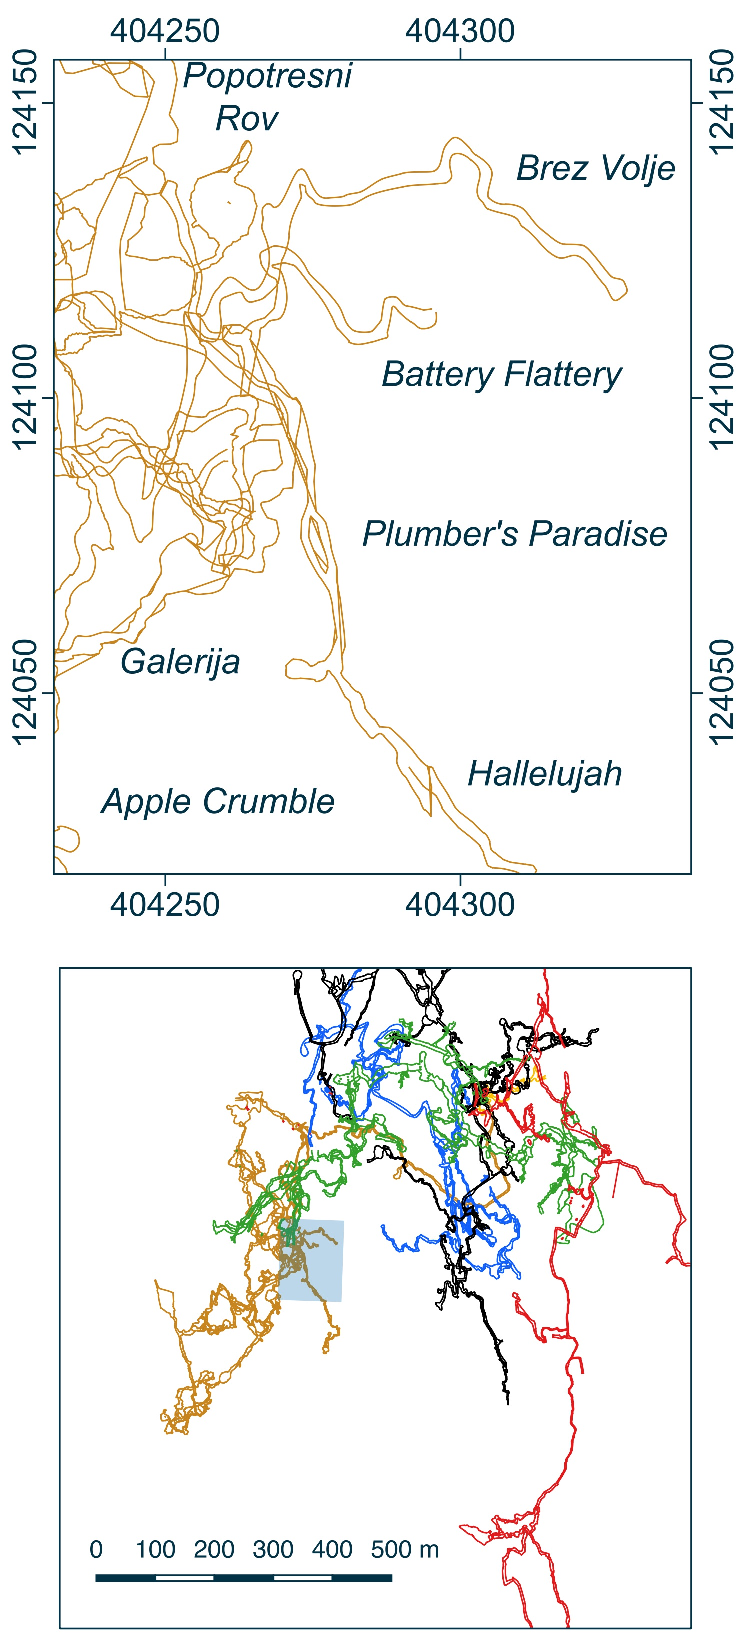
\includegraphics[width=\linewidth]{images/little_insets/hallelujah_inset.pdf}
 \caption*{Plan view of the \protect\passage{Hallelujah} branch. Slovenian National Grid ESPG 3794}
 \label{halleujah inset}
\end{marginfigure}

Clare lead for a few metres before stopping, giggling nervously. Ahead the passage was lined with dry mud, got tighter and turned a corner. She graciously allowed me the first go at it and I slipped down. I arrived in a delightful U-Bend and carried on. The passage continued, deliciously body sized, showing no sign of improvement. It was now my turn to giggle nervously as I approached a second u-bend almost full of soft mud. Clare’s echoey voice egged me on and I slid down. It was surprisingly dry and pleasant, and easy to wallow through. On the other side the passage continued. Another corner, a final  u-bend brought me into a chamber! I called back that it was going, encouraging Clare to join me. Then I heard Ben. 
‘Where are you?’ I called. 
‘Here’ he called back, helpfully. 
Rounding a corner I find him standing next to our body sized tube. Two leads crossed off for the price of one then.
 
Another lead beckoned and this time we encouraged Diss to take the first steps. A squeeze down into a slanted stoop that gradually deteriorated to an awkward crawl. A collapsed chamber offered us no easier going and I overtook Diss eventually finding another muddy crawl with the same soft, dry mud. There was not enough airspace above the mud to fit into but it was soft enough that a sort of breast stroke motion was enough to make progress. 10 meters in I could see the passage continuing for at least as long in front of me with no sign of improvement. Visions of a hell in which I was forced to swim through mud for eternity flicked across my mind and I decided I’d had enough, despite an encouraging draught.
 
We surveyed out, naming our find '\passage[lead]{Union Passage of the Year Nominee}', in recognition of a similar honour we had received from the Imperial College Union. On our way out Clare and I noticed a hole in the wall of the crawl, that popped out into a medium sized pitch and agreed that it should be checked out on our next visit. In total we’d left two undescended pitches and two going crawls. Not bad.
 
\begin{marginfigure}
 \begin{tikzpicture}
\node [name-dest] (box){%
    \begin{minipage}{0.80\textwidth}
    \begin{itemize}
    \item Rhys Tyers
    \item Ben Honan
    \item Clare Tan
    \end{itemize}
    \end{minipage}
};
\node[fancytitle, right=10pt] at (box.north west) {Plumber's Paradise};
\end{tikzpicture}
\end{marginfigure}
Ben, Clare and I returned the next day. With two batteries. Ben dropped the pitch we intended to drop the day before. Twenty metres down we landed on a rocky floor, a phreatic tube leading off behind some collapsed bits of wall. Ben had disappeared into it by the time Clare and I arrived so we scurried after him. We found him a few metres on. The tube was walking height and about the same width, very pleasant. The walls and floor were covered in the same sort of dryish mud we’d been wallowing in yesterday. We excitedly shook hands and stomped off down the passage.
 
Our elation was not to last though. We quickly arrived at a sump with no way on. The sump was beautifully clear, shimmering with a blue green tint but it represented the end of the lead for us so we were perhaps less awed by it than we should have been.
 
Ben and I surveyed out and Clare went to begin bolting the other pitch we’d found, off the crawl. Regrouping with Clare a little while later we found ourselves in a lovely clean shaft. Clare, with a classic “how is that even attached” deviation, threaded the rope down the pitch. At the bottom an awkward climb and grim crawl under a scary boulder rewarded the keen caver with another sump. This one had a ‘canal’ like feel as we couldn’t see the end from our vantage point. Clare tried to encourage me to wade in and check out the end but for some reason I wasn’t too keen.
 
  \begin{figure*}[t!]
\checkoddpage \ifoddpage \forcerectofloat \else \forceversofloat \fi
\centering
\begin{subfigure}[t]{0.495\textwidth}
\centering
\frame{\includegraphics[width=\linewidth]{"images/2017/rhys-hallelujah-2017/hallelujah".jpg}}
 \caption{}\label{water hallelujah}
\end{subfigure}
    \hfill
    \begin{subfigure}[t]{0.495\textwidth}
        \centering
        \frame{\includegraphics[width=\linewidth]{"images/2017/rhys-hallelujah-2017/diss-hallelujah".jpg}} 
        \caption{} \label{Diss and Dave}
    \end{subfigure}
    \caption{
    \emph{a} Dave Kirkpatrik bridging the stream canyon of \passage{Hallelujah}
    \emph{b} Rebecca Diss and Dave Kirkpatrik standing in \passage{Plumber's Paradise} passage --- Rhys Tyers}
\end{figure*}
 
We were tired and unenthusiastic at this point. The only way on we could see was a barely human sized section in a rift halfway up on the opposite wall. I think we were all ready to call it a day but we had 4 bolts left and I’d rather stick them in the wall than carry them out. I climbed up the wall on one side and rigged a traverse into the rift, showering Clare, who was relieving herself directly below me (better than the other way round I guess), with rock dust. It was tight and the rope was mostly for protecting this initial entry. Within the anthropic level continued for 4 metres before narrowing. Just before this though the rift below opened up just enough to get through, and a larger space beyond called to me. With my final two bolts I rigged a Y-hang in a place barely big enough to get the drill in horizontally. It’s really a collectors piece of a pitch head. The top is sort of hourglass shaped. You squeeze down to a sitting position below the rope, wiggle out along the rift a bit and carefully hold yourself in the widest bit as you descend. I was quite pleased when another of the expeditions experienced members said that it made him rethink what was possible to bolt.


 
I dropped a couple of metres to the floor and wandered forward. Another pitch! But about 10 metres down I could see water and I suspected it was the same water as the sump on the other side. I was out of bolts though and was about to turn around when I saw that the passage continued over the top of the pitch. A razor of rock sticking out from the wall as a step allowed me to carefully traverse over to it, still trailing the rope from my previous pitch behind. In front of me was another muddy phreatic tube! I was able to tie the rope off round a large pillar and called for the others to follow.

 
Having failed to learn from our previous mistakes we shook hands once again. We were sure this was it, hundreds of meters of easy walking passage straight to the lower entrance. We scurried along the stooping tube, excited as it enlarged to walking size. Then the sound of running water! We popped out in a stunning, white, clean streamway. About a metre wide and maybe 15 metres tall.


 
Here we quickly checked out upstream, finding a small muddy chamber above the stream and being unwilling to do the wet crawl required to follow the water. Then downstream. A lovely series of cascades led us to the end of our trip. The water did what it always does and disappeared into an impassable crack. Beyond the crack was a big space, and the water could be heard falling quite a distance on the other side so we consoled ourselves with the possibility of bring the plugs and feathers or heavier equipment here to break through.
 
We surveyed out, leaving the rope in because I promised to come back (Clare and Ben were both leaving in the next few days) and kill or continue it. As we surveyed out I pointed out that there could be ways on in the roof, it looked traversable higher up in the passage (oooh, foreshadowing). We named to streamway \passage{Hallelujah} and the rest '\passage{Plumbers Paradise}'.

 \begin{marginfigure}
 \begin{tikzpicture}
\node [name-dest] (box){%
    \begin{minipage}{0.80\textwidth}
    \begin{itemize}
    \item Rhys Tyers
    \item Dave Kirkpatrick
    \item Rebecca Diss
    \end{itemize}
    \end{minipage}
};
\node[fancytitle, right=10pt] at (box.north west) {Hallelujah};
\end{tikzpicture}
\end{marginfigure}  

I did return, several days later. Each day though weakened my resolve to break through the crack, each day it grew tighter and more impenetrable in my memory. The trip I ended up leading was a photo/derig trip as I had abandoned the plan to get through this year. Dave, Diss and I bimbled down to the pushing front taking photos along the way. As we prepared to derig I pointed out to Dave the place in the roof I thought might be traversable. Unusually he climbed the 2 metres straight away and without cajoling (he is normally very lazy). Once up there he nonchalantly called back “It goes. I think”.
  \begin{figure*}[t!]
\checkoddpage \ifoddpage \forcerectofloat \else \forceversofloat \fi
     \centering
        \frame{\includegraphics[width=\linewidth]{"images/2017/rhys-hallelujah-2017/diss-prima-hallelujah".jpg}} 
        \caption{ Rebecca Diss negotiates a climb above the stream canyon in \protect\passage{Hallelujah} ---  Rhys Tyers} \label{Diss Hallelujah}
\end{figure*} 
 
Diss and I shot up after him and, sending Diss in front, we found that it did indeed go. The ledges we climbed up on closed into form a solid floor, distinctly separating us from the streamway below. We rounded a couple of corners to confirm it didn’t die but it looked like we had a solid lead. Unfortunately we didn’t have a complete surveying kit and \bignote{being the good little cave explorers we are, we do not push without surveying}. We were excited though. Mostly because it meant we didn’t have to carry any rope out.
 
Two days later I was back again. Diss and I, armed with drills, rope, and surveying kit were ready. I was was certainly ready for a reward for all our efforts over the past few trips. The passage continued from where we left it, consistently about 3 metres high and a couple wide. Down a small climb (which on the way back required some combined tactics and a self-destructing escape cairn to climb up) we came to a pitch.
 \begin{marginfigure}
 \begin{tikzpicture}
\node [name-dest] (box){%
    \begin{minipage}{0.80\textwidth}
    \begin{itemize}
    \item Rhys Tyers
    \item Rebecca Diss
    \end{itemize}
    \end{minipage}
};
\node[fancytitle, right=10pt] at (box.north west) {Sweet Baby Jesus};
\end{tikzpicture}
\end{marginfigure}  
The passage intersected a large chamber. We dropped the 5 metres to the floor. Ignoring an obvious hole in the floor (still a lead!) we walked into the chamber and followed the passage on the other side. An alcove of stunning mud formations presented itself a we walked and we eventually came to a junction. The obvious continuation of the passage veered off to the right but a pleasant looking crawl headed straight on, due South. I was more interested in the crawl. \bignote{South means blank mountain. South means the lower entrance (eventually).} 
We popped up into the crawl. We encountered a vertical junction. Below, a lovely little canal which we elected not to explore and above a sandy squeeze. I do like a good squeeze and this was a stunning one. Smooth rock, sandy floor, just bigger than my Ecrin Rock on its side. Diss was leading up until that point but kindly let me go through first (seems to be a pattern). On the other side we found the other end of the canal (I think) and a small chamber, 1 metre high and 4 metres in diameter. Ahead the passage continued at stooping height, stunningly white and sandy, a series of stepped ledges leading off into the distance.
 

\begin{marginfigure}
\checkoddpage \ifoddpage \forcerectofloat \else \forceversofloat \fi
\centering
 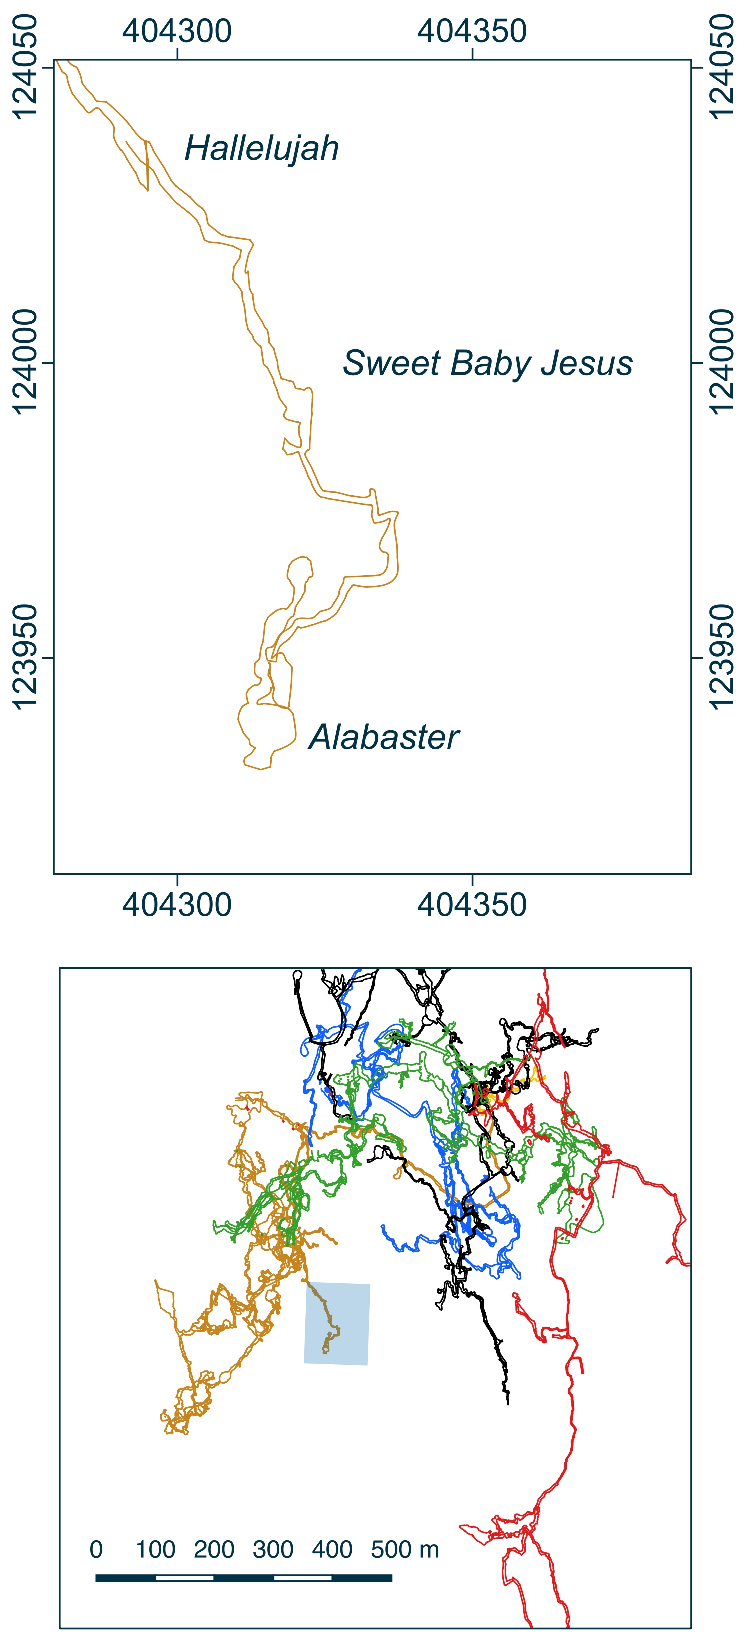
\includegraphics[width=\linewidth]{images/little_insets/sbj_inset.pdf}
 \caption*{Plan view of the \protect\passage{Hallelujah} branch. Slovenian National Grid ESPG 3794}
 \label{alabaster inset}
\end{marginfigure}

We turned back here. It was my last pushing trip of the expedition. One more team has been back (see Tanguy’s report on \passage[lead]{Alabaster}).
 
I don’t understand this lead at all. So many times it could have died but there was always a way through! Following an immature stream that disappeared into a crack we find a small window in a pitch. Here the obvious way on dies at a sump but a crawl has a tiny window into another pitch. The bottom of this pitch is sumped but there is just barely a passable level in a rift on the other side of the shaft. Beyond, its just possible to traverse into a passage that inexplicably becomes a muddy phreatic, which happens to join an active streamway! The streamway of course dies, but there happened to be a higher level! And straight into blank mountain!
 
This lead will certainly haunt my thoughts (and talk at the pub) until next year. Only 300 or so days to go.

\name{Rhys Tyers}
